\ShortPage{1. Host company}{
\subsection*{1.1 Profile and services}
\addcontentsline{toc}{subsection}{1.1 Profile and services}

CODELOGIC is a consulting firm specialized in software solutions [1]. It was
founded in 2023. Its services include custom software development, database
architecture, cloud solutions, security services, mobile development, and web
applications. The company also works on cloud and DevOps activities involving
continuous integration and delivery, scaling, and automation, as well as data
and API services involving secure integrations and data pipelines.

These activities place software construction, data management, deployment,
and integration in one service portfolio. Custom development addresses a
specific business need rather than a generic packaged product. Database
architecture concerns the organization and reliable access of application
data. Cloud and DevOps services concern repeatable delivery and operation.
Security services concern protection of systems and information. Mobile and
web development provide the application interfaces used by end users. Data
and API services connect information sources and software components.

My internship project was a Python and Flask data-analysis prototype connected
to the company's data, API, and web-application activities. It used stored
financial-market records and produced a complete analytical workflow, from
data preparation and statistical calculations to review files and browser
interfaces. This gave the assignment a clear place within CODELOGIC's software
solutions activity. The original prototype's browser dashboard was
later replaced by the React Terminal in the final project.

\keybox{\textbf{Company supervisor:} Firas Jebari.}

\subsection*{1.2 Internship setting and experience}
\addcontentsline{toc}{subsection}{1.2 Internship setting and experience}

My internship experience was organized around a complete technical assignment
rather than an isolated programming exercise. I worked with stored financial
data, Python analysis modules, generated CSV files, Flask endpoints, and a web
dashboard. The work required me to understand how each component contributed
to the final result and how information moved from a source row to an analyst's
screen.

I prepared and checked data, implemented statistical calculations, examined
unexpected outputs, connected results with news context, and presented the
generated evidence through clear interfaces. I also documented the processing
rules and verified them with automated tests. This combination made the
project both analytical and software-oriented.

The experience strengthened my autonomy and my attention to traceability. I
learned to record assumptions beside calculations, follow a displayed result
back to its source fields, and investigate an unusual value before changing a
rule. Financial data required precise interpretation because a large movement
could be statistically unusual without proving its cause.

Working on the prototype improved my ability to connect data preparation,
statistical reasoning, backend development, interface design, testing, and
technical writing. It also taught me to present a result in a form that another
person could review: the displayed value, the rule that selected it, the
available context, and the limits of the conclusion all had to remain visible.
}

\ShortPage{2. Introduction and project mission}{
The project is a statistical screening workflow for the Bourse des Valeurs
Mobilières de Tunis (BVMT), the Tunis Stock Exchange. It processes OHLCV data,
meaning the open, high, low, close, and traded volume recorded for each market
observation. It also uses stored headlines from ilboursa, a Tunisian financial
news website, as contextual evidence.

The central task was to reduce a large history of market observations to a
reviewable queue without turning an unusual movement into a legal conclusion.
For each symbol, the detector compares price returns and volume with earlier
observations. A z-score is the difference between an observed value and its
rolling mean, divided by the rolling standard deviation. It expresses how far
the value lies from that local reference in standard-deviation units.

The workflow separates four questions. First, is the volume unusual for this
symbol? Second, is the close-to-close return unusual? Third, is there a stored
headline for the same symbol near the flag date? Fourth, does the row satisfy
the narrow watchlist rule? These stages preserve the reason for each result.

The system is designed for a human analyst. A flag is a prompt to inspect the
market series and source context. A news match supplies context but does not
prove causation. The absence of a match means only that the stored news file
contains no qualifying same-symbol item within the search interval. The
project's practical value is the screening, news-context, watchlist, and
dashboard workflow rather than demonstrated detection accuracy.
}

\ShortPage{3. Data and processing pipeline}{
The market dataset contains 67,035 observations for 85 stored series (83 company shares plus PX1 and TBIDX).
dates run from 17 June 2021 to 12 October 2026. The combined news file contains
12,498 deduplicated records for 90 symbols, with valid dates from 29 February
2012 to 12 October 2026. Market and news universes differ because the two
collections do not cover exactly the same symbols.

\begin{center}
\captionof{table}{Stored analysis datasets}
\label{tab:short-datasets}
\small
\begin{tabularx}{\linewidth}{@{}lrrX@{}}
\toprule
Dataset & Rows & Symbols & Stored range and fields \\
\midrule
Market & 67,035 & 85 & 17 Jun 2021--12 Oct 2026; name, symbol, date, OHLCV \\
News & 12,498 & 90 & 29 Feb 2012--12 Oct 2026; symbol, date, time, headline, URL \\
\bottomrule
\end{tabularx}
\end{center}

Figure~\ref{fig:short-pipeline} summarizes the processing sequence.

\begin{center}
\begin{tikzpicture}[
  node distance=5mm and 8mm,
  box/.style={draw=blue,rounded corners,fill=softblue,align=center,
    minimum width=31mm,minimum height=10mm,font=\small},
  arrow/.style={-{Latex[length=2mm]},thick,color=blue}
]
\node[box] (raw) {Ticker OHLCV\\and news CSVs};
\node[box,right=of raw] (combine) {Validated\\combined files};
\node[box,right=of combine] (detect) {Spike and\\decay detectors};
\node[box,below=of detect] (context) {News context\\and categories};
\node[box,left=of context] (watch) {Watchlist and\\market context};
\node[box,left=of watch] (serve) {Flask APIs and\\React Terminal};
\draw[arrow] (raw) -- (combine);
\draw[arrow] (combine) -- (detect);
\draw[arrow] (detect) -- (context);
\draw[arrow] (context) -- (watch);
\draw[arrow] (watch) -- (serve);
\draw[arrow] (watch.south) -- ++(0,-6mm) -| node[pos=.25,below,font=\scriptsize]{evaluation} (serve.south);
\end{tikzpicture}
\captionof{figure}{Processing pipeline from stored market and news data to analyst-facing outputs.}
\label{fig:short-pipeline}
\end{center}

Analysis preserves the protected per-symbol market and news files. Derived CSV
files make each stage inspectable. Returns across gaps longer than ten calendar
days are omitted, and source OHLC values remain unchanged while quality issues
are written to a separate review file.

\subsection*{Data integrity and traceability}

The market loader parses dates and the numeric open, high, low, close, and
volume fields, then processes each symbol in date order. It checks missing or
non-numeric values, negative values, and inconsistent price ranges. The raw
policy records any issue in an audit table but does not repair the source row.
This separation is important because a correction chosen only to improve a
signal would make the analysis difficult to defend. A return is also set to
missing when two adjacent stored observations are more than ten calendar days
apart. The next score then draws its reference from 60 valid earlier returns
instead of treating a long inactive interval as a one-day price move.

News records are normalized by symbol and publication date and are
deduplicated before matching. The context stage never changes a flag. It adds
the selected headline, URL, timing status, gap in days, and category to a copy
of the detector output. This produces an explicit chain from a protected input
row to a statistical flag, a context record, a possible watchlist row, and an
evaluation result. The manifest stores hashes for the generated evaluation
inputs and outputs, so a report result can be checked against the exact files
that produced it.
}

\ShortPage{4. Statistical detector}{
For symbol $i$ and observation $t$, the detector uses log-volume
$x_{i,t}=\log(1+V_{i,t})$ and close-to-close return
$r_{i,t}=(P_{i,t}-P_{i,t-1})/P_{i,t-1}$. For either series
$q\in\{x,r\}$, the reference uses the previous 60 valid observations:
\[
 \mu^{q}_{i,t}=\frac{1}{60}\sum_{j=1}^{60}q_{i,t-j},\qquad
 s^{q}_{i,t}=\sqrt{\frac{1}{59}\sum_{j=1}^{60}
   \left(q_{i,t-j}-\mu^{q}_{i,t}\right)^2}.
\]
The full score is
\[
 z^{q}_{i,t}=\frac{q_{i,t}-\mu^{q}_{i,t}}
 {\max\!\left(s^{q}_{i,t},f_q\right)},
 \qquad f_x=0.10,\quad f_r=0.01.
\]
The observation at $t$ is excluded from its own mean and standard deviation.
For returns, invalid long-gap values are removed before the 60 valid prior
returns are selected.

\begin{center}
\captionof{table}{Detector parameters and rules}
\label{tab:short-detector}
\small
\begin{tabularx}{\linewidth}{@{}l l X@{}}
\toprule
Parameter & Value & Rule \\
\midrule
Reference length & 60 & Prior valid observations; observed row excluded \\
Volume threshold & $z^V>3.0$ & One-sided high-volume flag \\
Return threshold & $|z^R|>3.0$ & Two-sided price-return flag \\
Log-volume floor & 0.10 & Minimum denominator for volume score \\
Return floor & 0.01 & Minimum denominator for return score \\
Gap limit & 10 days & Longer-gap return is omitted \\
OHLC policy & Raw & Source values retained; issues logged \\
\bottomrule
\end{tabularx}
\end{center}

A union flag requires either the volume or return rule. A combined flag
requires both on the same row. The thresholds and 60-observation reference are
fixed in the source and were not selected from the labeled events.
}

\ShortPage{5. Flag output and worked examples}{
The frozen reference detector produces 1,414 union flags across 81 of the 85 stored series. There are
198 volume flags and 1,237 price flags. The 21 combined rows are counted in both signal
columns, so the counts reconcile as $198+1,237-21=1,414$.

Two stored rows illustrate the meaning of the fields. GIF on 22 October 2024
closed at 0.44 TND after a 10.00\% return. Its volume z-score was 1.341 and its
return z-score was 5.236. It was therefore a price-only flag, with no local
news match. It did not enter the watchlist because the rule requires both
signals. This row is also the only detector hit inside the primary window of a
source-backed event.

Carthage Cement (CC) on 30 October 2024 closed at 2.24 TND with volume
3,343,436 and a 5.660\% return. Its volume z-score was 4.069 and its return
z-score was 4.558. Both signals were true and no local news match was found, so
the row entered the spike route of the watchlist.

Figure~\ref{fig:short-anomalies} shows how these fields are presented as a
filterable review queue rather than as a verdict.

\reportfigure[0.50\textheight]{anomaly-feed.jpg}{fig:short-anomalies}{Anomaly Feed: stored flag dates, symbols, signals, and scores.}
}

\ShortPage{6. News context and watchlist funnel}{
The classification stage finds a same-symbol news item within seven calendar
days before or after each spike flag. It records whether a headline was
available by the flag date or appeared later. Of the 1,414 flags, 548 have a
local news match and 866 do not. The matched categories contain 311 other-news
rows, 200 earnings rows, 18 dividend rows, 13 governance rows, four capital
increase rows, one buyout row, and one suspension row.

The watchlist requires a combined price-and-volume flag with no local news
match. The mutually exclusive funnel accounts for every union flag:

\begin{center}
\captionof{table}{Mutually exclusive watchlist funnel}
\label{tab:short-funnel}
\small
\begin{tabularx}{\linewidth}{@{}Xr@{}}
\toprule
Outcome & Flags \\
\midrule
Single signal only, without a news match & 856 \\
Combined signal, but with a news match & 11 \\
Single signal and a news match & 537 \\
Combined signal, without a news match & 10 \\
\midrule
Total & 1,414 \\
\bottomrule
\end{tabularx}
\end{center}

The ten surviving spike flags join six unexplained decay cases, producing the
16-row refined watchlist. Ten other decay cases have a news match and do not
enter that queue. Figure~\ref{fig:short-watchlist} shows the retained rows and
their broad-market context tags.

\reportfigure[0.50\textheight]{watchlist.jpg}{fig:short-watchlist}{Watchlist: ranked dates and instruments in the refined queue.}
}

\ShortPage{7. Terminal review workflow}{
The final interface is a React, TypeScript, and Tailwind Terminal served at
\code{/} by the same read-only Flask API. The earlier seven-page template
dashboard was replaced. The seven current views are Overview, Anomaly Feed,
Stock Detail, News, Watchlist, Pipeline, and Evaluation.

Overview includes the Market Map. Its 83 company tiles are sized by average
traded value over the most recent 20 stored sessions, not market
capitalization. PX1 and TBIDX are index series, not company tiles. A symbol
without a trade on the aggregate as-of date is grey; an amber outline marks a
recent flag. The map and navigation support keyboard use and reduced-motion
preferences. The signal inspector opens the selected symbol's market and flag
context without changing the underlying records.

\reportfigure[0.37\textheight]{overview-market-map.jpg}{fig:short-overview}{Overview: Market Map controls and sample tiles from 83 companies.}
\reportfigure[0.37\textheight]{inspector-open.jpg}{fig:short-inspector}{BIAT signal inspector: detector scores and rule explanation.}
}

\ShortPage{8. Skills and lessons learned}{
The internship developed my ability to connect statistical reasoning with a
complete software workflow. I learned to prepare and validate data with
Python and pandas, calculate grouped time-series indicators, expose derived
results through Flask endpoints, and present them in a browser interface. I
also learned that an implementation is not complete until its outputs can be
traced, tested, and explained.

\subsection*{Technical learning}

The detector made temporal order concrete. An observation must not enter its
own reference window, a long trading gap must not be treated as an ordinary
daily return, and missing values must be handled without silently changing the
meaning of later scores. Working through these cases strengthened my knowledge
of rolling statistics, date handling, grouped processing, and data-quality
controls.

Building the dashboard taught me how the backend and interface depend on the
same data contract. Each JSON field had to preserve the symbol, date, score,
news status, and selection rule used in the generated files. I also improved
the data-loading layer with modification-time caches. This showed me how to
improve responsiveness while preserving identical returned information and
automatic reloads when a file changes.

\subsection*{Analytical and professional learning}

The most important analytical lesson was to separate detection, context, and
conclusion. A statistical flag identifies an unusual observation; a nearby
headline adds context; neither proves causation or intent. The limited event
register also taught me to report a small case study honestly instead of
generalizing from a small sourced event set with one held-out positive.

Professionally, I became more autonomous in breaking a large assignment into
verifiable stages. I learned to investigate unexpected values before changing
a rule, document assumptions beside the relevant calculation, use automated
tests to protect earlier work, and communicate limitations as clearly as
results. These habits are transferable to other data-analysis and software
projects.
}

\ShortPage{9. Evaluation and limitations}{
\small
The frozen \code{reference_v1} still produces 1,414 flags: 1,399
on company shares and 15 on PX1, with none on TBIDX. It hits one of
the original three sourced events. The Phase 2 protocol was committed before
candidate code and expanded-label hit tables. Its sourced registry gained 18
rows; after the audit, these are 13 negative controls, three exploratory
rows, and two positives. Seven positive rows have dated source URLs;
the evaluation source metric excludes unlisted TSI through its headline-
inclusion rule and counts six. Five have primary-window trading coverage.
Four covered positives fall in development
(before 2025-01-01) and one in the held-out period. The primary window is
30 days before to five days after public disclosure; the secondary starts
60 days before. These are screening case studies, not accuracy estimates.

The reference hits 1/4 development positives (95\% Wilson 0.05--0.70) and
0/1 held-out positives (0.00--0.79). Across all five it hits 1/5
(0.04--0.62) in the primary window and 2/5 in the secondary. Workload is
4.08 and 7.12 flags per observed calendar week in the two splits. The
development-selected robust candidate hits 2/4 but 0/1 held out, produces
10.83 and 21.94 flags per week, and fails the predeclared adoption rule.
The simple volume-spike baseline hits 4/4 and 1/1, but at 16.87 and
24.38 flags per week, about four times the reference workload; its 27 and
10 control flags also exceed the reference's 4 and 9. Hit count alone is
not an advantage. No candidate met the baseline and
workload requirements. The decision remains to retain \code{reference_v1}.

For $k$ hits in $n$ events, the implemented two-sided Wilson interval
uses $z=1.959963984540054$, $\hat p=k/n$, and $D=1+z^2/n$.
The centre and half-width are
\[C=\frac{\hat p+z^2/(2n)}{D},\qquad
H=\frac{z\sqrt{\hat p(1-\hat p)/n+z^2/(4n^2)}}{D}.\]
Bounds are $\max(0,C-H)$ and $\min(1,C+H)$.
The robust score uses the prior 60 valid values:
$z^{rob}_t=(q_t-\operatorname{median}(q_{<t}))/
\max(1.4826\operatorname{MAD}(q_{<t}),f)$.
Abnormal return is $r^{stock}_t-r^{PX1}_t$ on an exact matching date.
For 1,000 same-count-per-symbol random placements, the one-sided
permutation value is $(1+\#\{h_b\geq h_{actual}\})/1001$.

Six registered candidates test robust median/MAD scores at cutoffs 3 and 4,
market-adjusted returns, an activity filter, a persistence rule, and
point-in-time decay. Comparators include volume only, return only, a simple
volume spike, top two per month, and same-count random placement. Candidate
flags do not rewrite the frozen reference output.

The source audit moved UADH's suspension anchor to 25 March 2026, labeled
Syphax's 19 December 2023 report as a public announcement (the court ruling
was 11 December), and moved ADWYA's reason-undisclosed suspension to
exploratory rather than a negative control. PGH and LNDOR share one notice,
so control flags are shown both separately and with that notice collapsed.
No method's event hit status changed after these corrections. The quality
review found zero duplicate symbol/date rows, zero invalid dates, 59 invalid
numeric or OHLC rows, 349 long gaps, and 115 possible corporate-action
rows for human review. The held-out positive count is one, labels are
incomplete, and no human classifier-agreement result is available.

\begin{center}
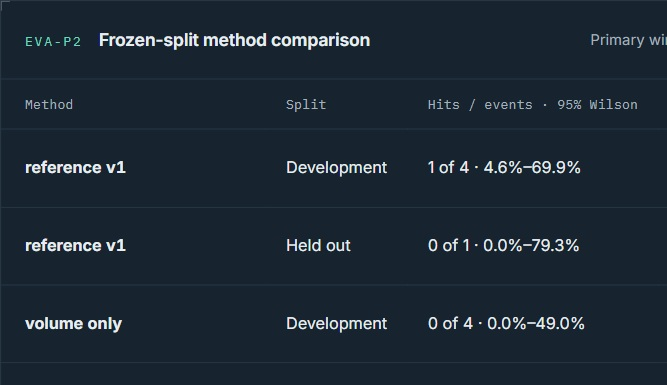
\includegraphics[width=\linewidth,height=0.36\textheight,keepaspectratio]{evaluation.jpg}
\captionof{figure}{Evaluation: reference and baseline hit comparisons.}
\label{fig:short-evaluation}
\end{center}
}
\ShortPage{10. Conclusion}{
The final project combines stored BVMT market and ilboursa news records,
prior-only statistical screening, a refined review queue, source-audited
evaluation, and a React Terminal served by Flask. The project was continued
after the internship period with the agreement of the company supervisor.
The cover retains the internship dates of 1 July to 1 August 2026.

The frozen reference produces 1,414 flags. Its result remains one hit
among the original three sourced positives and one among five eligible
positives in the expanded primary window. The sole held-out positive is
a miss. Six candidate variants were evaluated without retuning; none
met the adoption rule, so \code{reference_v1} remains the selected
method. The small event register cannot support a general accuracy
estimate or a misconduct conclusion.

The Terminal connects each displayed signal to stored market values,
flag fields, news context, and selection rules. At the time of final
verification, the offline suite passed 117 tests; the React build and
format check passed. Remaining limitations include thin trading,
unadjusted prices, incomplete event labels, one stored news source,
and only one held-out positive. Human review remains essential.

\subsection*{References}
[1] CODELOGIC, company presentation, \texttt{https://www.codelogic.tn}.
[2] Project repository: Phase 2 results and protocol, final event register,
and generated method comparison.
}
